\item A uniform solid cylinder with radius R and length L has moment inertia $I_1$, about the axis of the cylinder. A concentric solid cylinder of radius $R' = \frac{R}{2}$ and length $L' = \frac{L}{2}$ is carved out of the original cylinder. If $I_2$ is the moment of inertia of the carved out portion of the cylinder then $\frac{I_1}{I_2}$ =
        \underline{\hspace{2.5cm}}.
    \begin{center}
        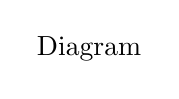
\begin{tikzpicture}
            \node at (0, 0) {Diagram};
        \end{tikzpicture}
    \end{center}
(Both $I_1$ and $I_2$ are about the axis of the cylinder)